\documentclass{article}

\usepackage{graphicx}
\usepackage{tikz}
\usepackage{tikzsymbols}
\usetikzlibrary{calc,patterns,shapes.geometric}
\pagestyle{empty}
\usepackage[margin=0pt]{geometry}
\geometry{papersize={14in,12in}}

\def\centerarc[#1](#2)(#3:#4:#5){\draw[#1] ($(#2)+({#5*cos(#3)},{#5*sin(#3)})$) arc (#3:#4:#5);}

\begin{document}
	\begin{figure}
		\centering
		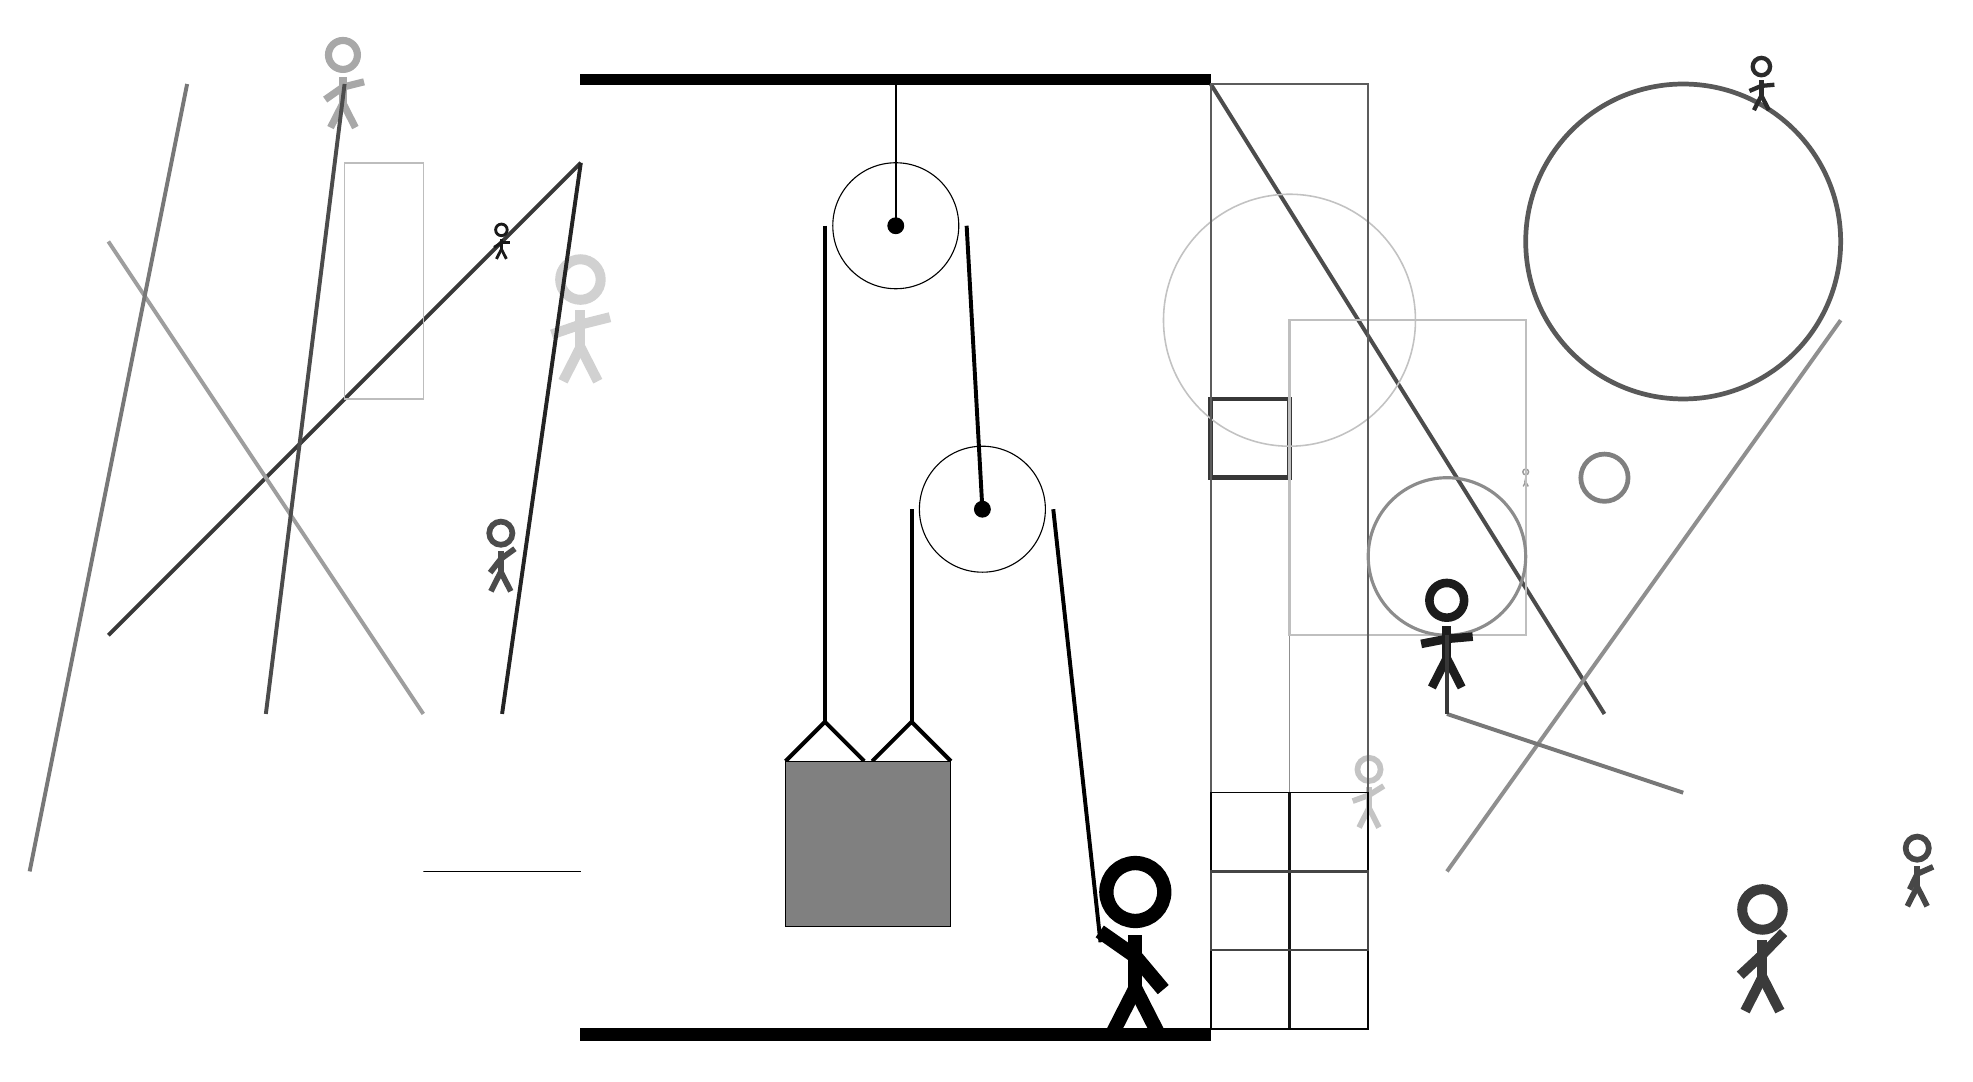
\begin{tikzpicture}
			%%%%% START %%%%%
			
			\draw[fill=black] (-2, 9) rectangle (6, 9.125);
			
			\draw (2, 7.2) circle (0.8);
			\draw[fill=black] (2, 7.2) circle (0.1);
			\draw[thick] (2, 7.2) -- (2, 9);
			
			\draw[line width=0.5mm, color=black!70](11, 1) -- (6, 9);
			
			\draw[line width=0.5mm, color=black!78](-2, 8) -- (-8, 2);
			\draw[line width=0.2mm, color=black!44] (7, 6) rectangle (8, -1);
			\node[line width=0.2mm, color=black!40] at (10, 4) {\Strichmaxerl[1][77][80]};
			\draw[line width=0.5mm, color=black!44](9, -1) -- (14, 6);
			
			\node[line width=0.4mm, color=black!34] at (-5, 9) {\Strichmaxerl[5][35][14]};
			\draw[line width=0.6mm, color=black!78] (6, 5) rectangle (7, 4);
			\node[line width=0.4mm, color=black!18] at (-2, 6) {\Strichmaxerl[7][19][14]};
			\draw [line width=0.2mm, color=black!24](7, 6) circle (1.6);
			\node[line width=0.4mm, color=black!23] at (8, 0) {\Strichmaxerl[4][20][32]};
			\draw[line width=0.5mm, color=black!38](-4, 1) -- (-8, 7);
			\draw[line width=0.3mm, color=black!25] (7, 2) rectangle (10, 6);
			\draw[line width=0.5mm, color=black!70](-6, 1) -- (-5, 9);
			
			\draw[line width=0.5mm, color=black!86](-3, 1) -- (-2, 8);
			\draw[line width=0.3mm, color=black!64] (8, -1) rectangle (6, 9);
			\draw [line width=0.6mm, color=black!50](11, 4) circle (0.3);
			
			\node[line width=0.2mm, color=black!77] at (13, -2) {\Strichmaxerl[7][43][46]};
			\node[line width=0.6mm, color=black!72] at (15, -1) {\Strichmaxerl[4][64][24]};
			\draw[line width=0.2mm, color=black!100] (-2, -1) rectangle (-4, -1);
			
			\draw [line width=0.4mm, color=black!45](9, 3) circle (1.0);
			\draw[line width=0.5mm, color=black!92](7, 0) -- (7, -3);
			\node[line width=0.5mm, color=black!90] at (-3, 7) {\Strichmaxerl[2][32][0]};
			
			\draw[line width=0.2mm, color=black!98] (8, -3) rectangle (6, 0);
			\draw[line width=0.5mm, color=black!53](9, 1) -- (12, 0);
			\draw [line width=0.6mm, color=black!65](12, 7) circle (2.0);
			
			\draw[line width=0.3mm, color=black!73] (6, -1) rectangle (8, -2);
			
			\node[line width=0.6mm, color=black!70] at (-3, 3) {\Strichmaxerl[4][52][36]};
			\draw[line width=0.5mm, color=black!53](-7, 9) -- (-9, -1);
			\node[line width=0.7mm, color=black!89] at (9, 2) {\Strichmaxerl[6][11][5]};
			\draw[line width=0.2mm, color=black!26] (-4, 5) rectangle (-5, 8);
			\node[line width=0.3mm, color=black!83] at (13, 9) {\Strichmaxerl[3][23][5]};
			\draw[line width=0.5mm, color=black!78](9, 2) -- (9, 1);
			
			\draw (3.1, 3.6) circle (0.8);
			\draw[fill=black] (3.1, 3.6) circle (0.1);
			
			\draw[line width = 0.5mm]  (0.6, 0.4) -- (1.1, 0.9) -- (1.6, 0.4);
			\draw[line width = 0.5mm]  (1.7, 0.4) -- (2.2, 0.9) -- (2.7, 0.4);
			\draw[fill=black!50] (0.6, 0.4) rectangle (2.7, -1.7);
			
			\draw[line width = 0.5mm] (1.1, 7.2) -- (1.1, 0.9);
			\centerarc[line width = 0.5mm](2, 7.2)(0:180:0.9);
			\draw[line width = 0.5mm] (2.9, 7.2) -- (3.1, 3.6);
			\draw[line width = 0.5mm] (2.2, 3.6) -- (2.2, 0.9);
			\centerarc[line width = 0.5mm](3.1, 3.6)(0:180:0.9);
			\draw[line width = 0.5mm] (4.0, 3.6) -- (4.6, -1.9);
			
			\node at (5, -2) {\Strichmaxerl[10][-35][-50]};
			
			\draw[fill=black] (-2, -3) rectangle (6, -3.15);
			
			%%%%% END %%%%%
		\end{tikzpicture}
	\end{figure}	
\end{document}